% Figures/separation.tex
% Illustrates Definition \ref{def:hyperplane}, Theorem \ref{thm:separation-2}
% (strict separation) and Theorem \ref{thm:supporting-hyperplane} of Chapter
% \ref{ch:convexity}.
% Source: Fukuda (2026), Supplementary Ch. 10, Sec. 10.2 (pp. 334-345).
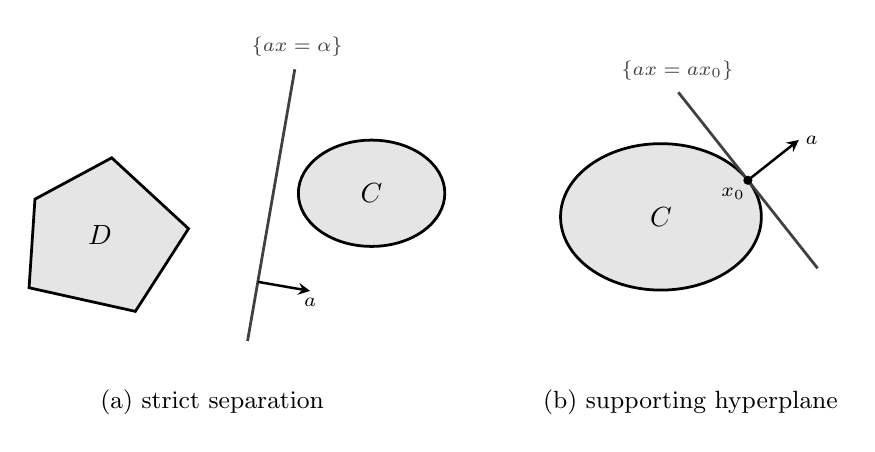
\begin{tikzpicture}[
		scale=1.5,
		>=stealth,
		setline/.style={line width=1pt,black,fill=black!10},
		hyper/.style={line width=1pt,black!75},
		normalarrow/.style={->,line width=0.9pt,black},
		panel/.style={font=\small},
	]

	% ---------- panel A: strict separation ----------
	\begin{scope}
		\filldraw[setline] (0.15,0.35) -- (1.05,0.15) -- (1.50,0.85) --
		(0.85,1.45) -- (0.20,1.10) -- cycle;
		\node at (0.75,0.80) {$D$};
		\filldraw[setline] (3.05,1.15) ellipse [x radius=0.62, y radius=0.45];
		\node at (3.05,1.15) {$C$};
		\draw[hyper] (2.00,-0.10) -- (2.40,2.20);
		\node[hyper,anchor=south,font=\scriptsize] at (2.42,2.22)
		{$\{\ip{a}{x}=\alpha\}$};
		\draw[normalarrow] (2.087,0.40) -- ++(0.443,-0.077)
		node[below,font=\scriptsize,inner sep=2pt] {$a$};
		\node[panel] at (1.70,-0.62) {(a) strict separation};
	\end{scope}

	% ---------- panel B: supporting hyperplane ----------
	\begin{scope}[shift={(4.30,0)}]
		\filldraw[setline] (1.20,0.95) ellipse [x radius=0.85, y radius=0.62];
		\node at (1.20,0.95) {$C$};
		\draw[hyper] (2.526,0.515) -- (1.347,2.005);
		\node[hyper,anchor=south,font=\scriptsize] at (1.34,2.02)
		{$\{\ip{a}{x}=\ip{a}{x_0}\}$};
		\fill (1.936,1.260) circle (1.1pt);
		\node[anchor=north east,font=\scriptsize,inner sep=1.5pt]
		at (1.95,1.235) {$x_0$};
		\draw[normalarrow] (1.936,1.260) -- ++(0.431,0.341)
		node[right,font=\scriptsize,inner sep=2pt] {$a$};
		\node[panel] at (1.45,-0.62) {(b) supporting hyperplane};
	\end{scope}

\end{tikzpicture}
